\section{Lo Strato di Trasporto}
Lo strato di trasporto dello stack protocollare TCP/IP presenta caratteristiche quali:
\begin{itemize}
    \item Realizzazione di \textcolor{purple}{comunicazioni logiche} fra processi residenti su host diversi. Logiche perché i processi si comportano come se gli host fossero direttamente collegati, ingorando i dettagli infrastrutturali.
    \item Offrire servizi di trasporto (per l'appunto) allo strato applicativo, che possono essere:
        \begin{itemize}
            \item \textcolor{blue}{Sequenze di messaggi singoli};
            \item \textcolor{blue}{Sequenza continua di byte}.
        \end{itemize}
        L'applicazione manda i dati al livello di trasporto, nella forma richiesta per la consegna.
    \item Sfrutta i servizi dello strato di rete che si occupa della comunicazione tra host e il quale consegna i datagrammi all'host destinatario (e non al processo).
\end{itemize}

\begin{figure}[h]
    \centering
    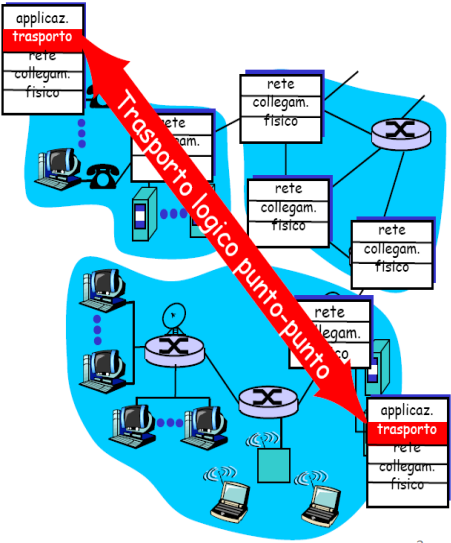
\includegraphics[scale=0.5]{Immagini/Lo_Strato_di_Trasporto.png}
    \caption{Lo strato di trasporto.}
\end{figure}

\newpage

\paragraph{Tipologie di Connessione}
Lo strato di trasporto offre principalmente due tipologie di servizio:
\begin{itemize}
    \item \textbf{\textcolor{purple}{Servizio privo di connessione:}} In questo caso il processo mittente di occupa di consegnare i \textcolor{blue}{messaggi} al livello di trasporto uno per uno e il livello di trasporto li considera in maniera indipendente, senza creare alcun tipo di relazione tra di essi. 
    \\In questa tipologia di servizio non vi sono garanzie di consegna o di ordinamento.
    \item \textbf{\textcolor{purple}{Servizio orientato alla connessione}} In questa tipologia di servizio il processo mittente e il processo destinazione vengono collegati mediante una \textcolor{blue}{connessione logica}.
\end{itemize}

I due principali protocolli messi a disposizione nel livello di trasporto, come detto nel capitolo precedente, sono TCP e UDP che vedremo poi in dettaglio.

\paragraph{Multiplexing e Demultiplexing}
Indipendentemente dal protocollo utilizzato, le azioni che vengono esequite durante le fasi di invio e ricezione dei segmenti sono le medesime:
\begin{itemize}
    \item Durante la fase di invio dei dati (\textcolor{purple}{Multiplexing}), il livello di trasporto riceve i messaggi dal livello applicativo, determina gli header per quel segmento, crea il segmento e invia il risultato al livello di rete (IP);
    \item Durante la fase di ricezione dei dati (\textcolor{purple}{Demultiplexing}), il livello di trasporto riceve i segmenti dal livello di rete, controlla i valori dell'header, estrae il messaggio e lo smista all'applicazione corretta attraverso la socket.
\end{itemize}

\paragraph{Concetto di Porta}
Ogni datagramma, presenta:
\begin{itemize}
    \item un indirizo IP sorgente e IP destinazione;
    \item un segmento del livello di trasporto, nel cui header sono presenti un numero di porta sorgente e un numero di porta destinazione.
\end{itemize}
Ogni comunicazione di trasporto è identificata in maniera univoca grazie alle coppie IP/porta degli host. Come visto in precedenza questi sono degli identificativi rispettivamente a 32 bit, per identificare l'host, e 16 bit, per identificare il processo sull'host. Il SO si occupa dell'assegnazione dinamica delle porte ai processi che ne fanno richiesta.
\\Esistono inoltre delle porte che sono assegnate arbitrariamente da IANA e che \underline{non} possono essere utilizzate liberamente dagli utenti o dalle applicazioni.

\paragraph{Demultiplexing con e senza connessione}
La fase di Demultiplexing dipende fortemente dal protocollo utilizzato. Nel caso del protocollo UDP le socket vengono identificate univocamente da una coppia IP/Porta, questo sta a significare che due datagrammi con IP e/o porta sorgente differenti ma medesima coppia IP/porta destinazione verranno consegnati alla stessa socket.

\begin{figure}[h]
    \centering
    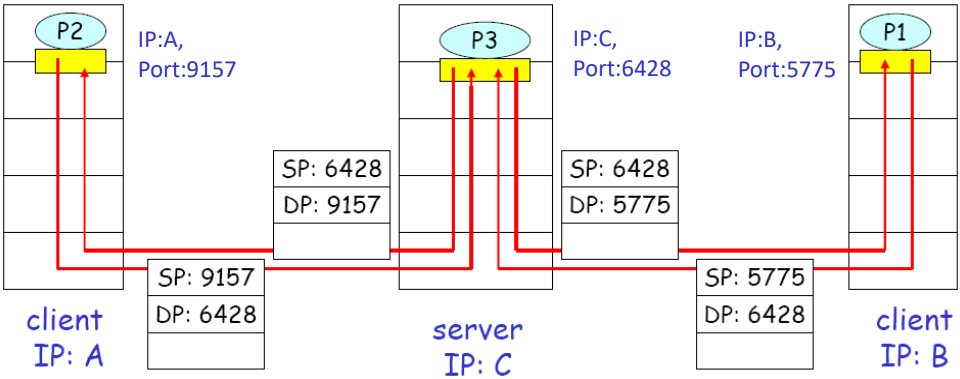
\includegraphics[scale=0.4]{Immagini/DemultiplexingUDP.png}
    \caption{Demultiplexing UDP.}
\end{figure}

Questo non è vero per le socket del protocollo TCP le quale vengono idetificate da una quadrupla data da:
\begin{itemize}
    \item Indirizzo IP di origine
    \item Numero di porta di origine
    \item Indirizzo IP di destinazione
    \item Numero di porta di destinazione
\end{itemize}
Una possibile consegnenza di ciò è che un host server può supportare più connessioni distinte contemporaneamente sulla stessa porta.

\begin{figure}[h]
    \centering
    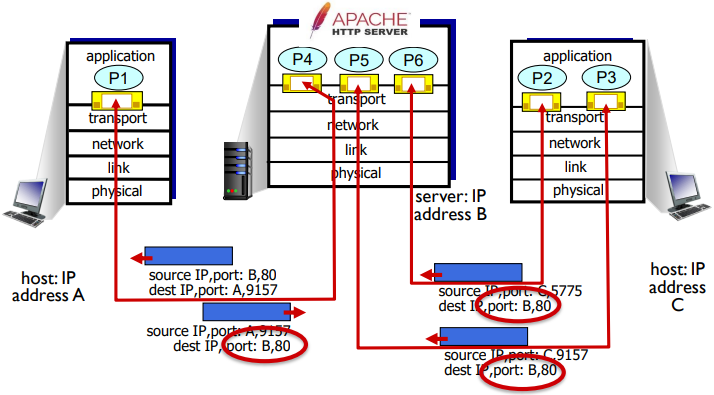
\includegraphics[scale=0.48]{Immagini/DemultiplexingTCP.png}
    \caption{Demultiplexing TCP.}
\end{figure}

\subsection{TCP}
Il protocollo TCP come detto è uno dei due principali protocolli offerti dal livello di trasporto.
Questo presenta una serie di proprietà quali:
\begin{itemize}
    \item \textbf{\textcolor{purple}{Orientamento allo stream:}} i dati vengono visti come un flusso continuo di byte ordinati, ma non strutturati. 
    La lunghezza di questo fullo è indefinita ma la macchina destinazione riceve esattamente la stessa sequenza di byte che la macchina mittente ha inviato.
    \item \textbf{\textcolor{purple}{Orientamento alla connessione:}} prima che avvenga lo scambio di dati i processi residenti sulle due macchine effettuano un \textcolor{purple}{handshake}, una procedura di scambio di informazioni preliminari. 
    \\Viene detto \textcolor{purple}{orientato} alla connessione perchè lo stato della connessione risiede sui punti terminali e non sugli elementi intermedi.
    TCP quindi fornisce agli \textcolor{blue}{USER} l'illusione di avere un circuito dedicato fornendo loro un servizio \textcolor{blue}{Connection Oriented}, basandosi però sul protocollo di rete IP il quale fornisce servizio un \textcolor{blue}{Connection Less}.
    \item \textbf{\textcolor{purple}{Connessione full-duplex:}} il flusso di dati tra due host può avvenire contemporaneamente nelle due direzioni; queste infatti sono slegate tra loro.
    \item \textbf{\textcolor{purple}{Trasferimento bufferizzato:}}TCP è in grado di suddividere il flusso di byte in segmenti in modo indipendente dal programma applicativo che li ha generati. 
    Appena i dati sono sufficienti per riempire un segmento ragionevolmente grande, questo viene trasmesso attraverso la rete. Ciò viene implementato tramite l'utilizzo di un buffer.
    \\La bufferizzazione consente una riduzione del traffico sulla rete "ottimizzando" in qualche modo il numero di segmenti da trasmettere.
    \item \textbf{\textcolor{purple}{Ordinamento e affidabilità:}}si intende la capacità di correggere errori quali:
    \begin{itemize}
        \item \textcolor{blue}{dati corrotti};
        \item \textcolor{blue}{segmenti persi};
        \item \textcolor{blue}{segmenti duplicati};
        \item \textcolor{blue}{segmenti fuori sequenza}.
    \end{itemize}
    Questo viene fatto tramite una serie di controlli:
    \begin{itemize}
        \item \textcolor{purple}{Controllo di sessione:} meccanismi di inizio e fine trasmissione;
        \item \textcolor{purple}{Controllo di flusso:} evitare di spedire più dati di quanti il ricevente sia in grado di trattare;
        \item \textcolor{purple}{Controllo di congestione:} ha lo scopo di recuperare situazioni di sovraccarico nella rete.
    \end{itemize}
    
\end{itemize}

\paragraph{Trasferimento bufferizzato}
I processi al livello applicativo che utliizzano TCP scrivono/leggono dal buffer (spessso a velocità diverse) ed essendo la comunicazione bidirezionale, entrambi i lati avranno un buffer di invio e un buffer di ricezione.
\begin{figure}[h]
    \centering
    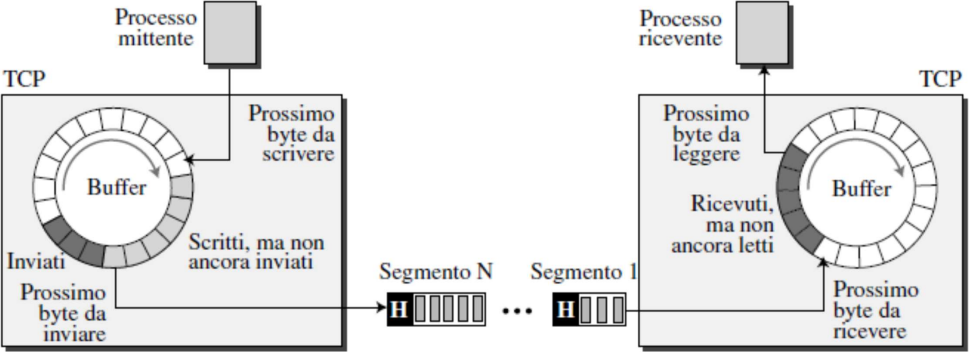
\includegraphics[scale=0.48]{Immagini/BufferizzazioneTCP.png}
    \caption{Bufferizzazione TCP.}
\end{figure}

Il flusso di byte viene partizionato in segmenti, oguno dei quali ha il suo header, i quali vengono poi consegnati al livello IP.

\subsubsection{Formato Segmento}
\begin{figure}[h]
    \centering
    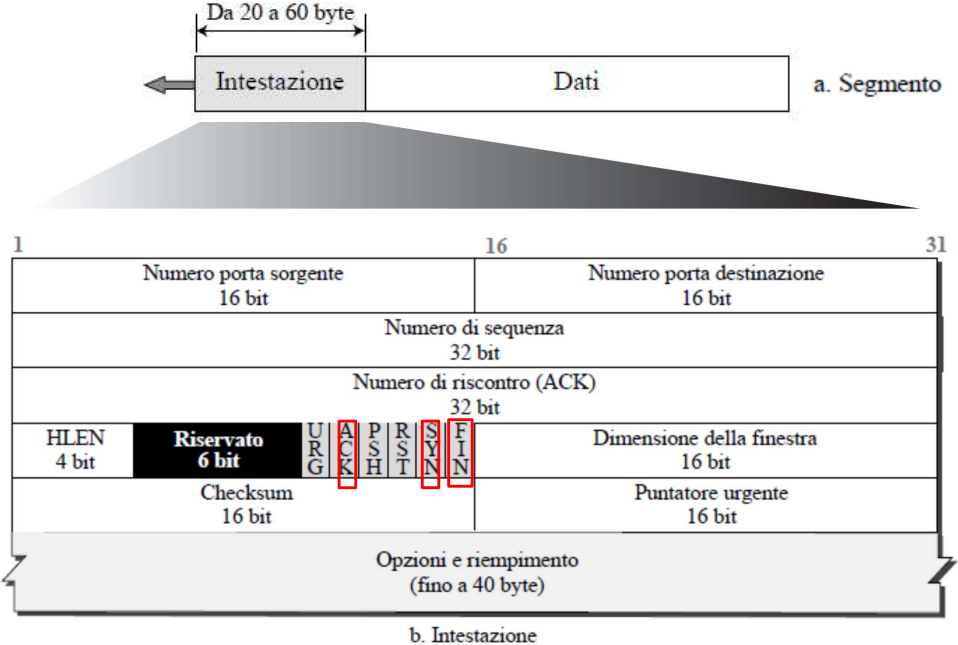
\includegraphics[scale=0.45]{Immagini/FormatoSegmentoTCP.png}
    \caption{Formato segmento TCP.}
\end{figure}

La semantica dei campi dei campi dell'header TCP è la seguente:
\begin{itemize}
    \item \textcolor{purple}{Numero di sequenza:} è il numero di sequenza nello stream del primo byte di dati di questo segmento. In TCP infatti vengono numerati i byte e non i segmenti, partendo da un numero casuale !=0. 
    Se il flag SYN è settato il numero di sequenza è \textcolor{purple}{ISN} (Initial Sequence Number) e il primo byte di dati è ISN+1.
    \item \textcolor{purple}{Numero di riscontro:} se il bit ACK è settato, questo campo contiene il valore del prossimo numero di sequenza che il mittente del segmento si aspetta di ricevere dall’altro host. 
    Una volta che la connessione è stabilita è sempre inviato.
    \item \textcolor{purple}{Finestra di ricezione:}  indica il numero di byte di dati a partire da quello indicato nel campo \textcolor{blue}{Numero di Riscontro} che il mittente di questo segmento è in grado di accettare. 
\end{itemize}

Questi tre campi sono essenziali in quanto permettono di realizzare il \textcolor{blue}{flow control}, il \textcolor{blue}{meccanismo di ritrasmissione} e il \textcolor{blue}{meccanismo di riordino} dei pacchetti in ricezione, necessari per la struttura stream-based del TCP.

\begin{itemize}
    \item \textcolor{purple}{Hlen:} lunghezza dell'header TCP espressa in parole da 4 byte.
    \item \textcolor{purple}{Checksum:} checksum dell'intero pacchetto (dati, header TCP e parte dell'header IP) che permette di rilevare errori.
    \item \textcolor{purple}{Puntatore Urgente:} questo campo è un offset positivo a partire dal \textcolor{blue}{Numero di Sequenza} del segmento corrente. 
    Punta al primo byte di dati \underline{non} urgenti a partire dal \textcolor{blue}{Numero di Sequenza}, e consente di far passare i dati urgenti in testa alla coda di ricezione. 
    Nel segmento contenente dati urgenti deve essere presente almeno un byte di dati.
    \item \textcolor{purple}{Bit codice:} sono 6 flag e servono per
        \begin{itemize}
            \item \textcolor{blue}{URG:} Il campo Puntatore Urgente è significativo e ci sono dati da trasferire in via prioritaria.
            \item \textcolor{blue}{ACK:} Il campo Numero di Riscontro contiene dati significativi.
            \item \textcolor{blue}{PSH:} Funzione Push (trasferimento immediato dei dati in un segmento dal trasporto al livello applicativo)
            \item \textcolor{blue}{RST:} Reset della connessione
            \item \textcolor{blue}{SYN:} Sincronizza il Numero di Sequenza
            \item \textcolor{blue}{FIN:} Non ci sono altri dati dal mittente, chiusura della connessione
        \end{itemize}
    \item \textcolor{purple}{Opzioni} \underline{(facoltativo, lunghezza variabile, max 40 byte)}: negoziazione di vari parametri; ad es. dimensione massima segmento (MSS), selective acknowledgement supportato e blocchi di dati riscontrati selettivamente. Le opzioni sono sempre multipli di 8 bit e il loro valore è considerato per il calcolo della checksum.
\end{itemize}

\subsubsection{Gestione della Connessione}